\documentclass[aps,pre,twocolumn,superscriptaddress,floatfix]{revtex4-2}

\usepackage{amsmath}
\usepackage{amssymb}
\usepackage{amsfonts}
\usepackage{graphicx}
\usepackage{dcolumn}
\usepackage{bm}
\usepackage{booktabs}
\usepackage{microtype}
\usepackage{hyperref}
\usepackage{xcolor}

\renewcommand{\topfraction}{0.95}
\renewcommand{\bottomfraction}{0.85}
\renewcommand{\textfraction}{0.05}
\renewcommand{\floatpagefraction}{0.8}

\hypersetup{
    colorlinks=true,
    linkcolor=blue,
    citecolor=blue,
    urlcolor=blue
}

\begin{document}

\title{Excess Entropy and Self-Diffusion in Multicomponent Charged Fluids: \texorpdfstring{\\}{} A Comparative Integral Equation and Molecular Dynamics Investigation}

\author{E. Lomba}
\email{e.lomba@csic.es}
\affiliation{Instituto de Qu{\'\i}mica F{\'\i}sica Blas Cabrera, CSIC, Serrano 119, E-28006 Madrid, Spain}

\date{\today}

\begin{abstract}
We investigate the excess entropy, structural two-body entropy, and transport properties of multicomponent charged Lennard-Jones mixtures along a supercritical isotherm ($T^* = 2.00$, $\Gamma = 1.0$) up to dense liquid packing ($\rho^* = 0.70$). We contrast a symmetric 3-component electrolyte mixture (neutral solvent with a 2:2 salt, ionic strength $I = 0.40$) against an asymmetric 5-component mixture (neutral solvent with mixed 1:1 and 2:2 salts at identical total packing fraction $\eta \approx 0.3665$, but lower ionic strength $I = 0.19$). Hypernetted Chain (HNC) integral equation theory incorporating Allnatt electrostatic screening is evaluated alongside extensive GPU-accelerated molecular dynamics simulations across 15 density points. We demonstrate that numerical differentiation of the HNC excess free energy functional rigorously reproduces the virial compressibility factor ($Z_{\text{diff}} \equiv Z_{\text{virial}}$) across the entire density range, confirming internal Euler thermodynamic consistency. Furthermore, thermodynamic integration of the MD pressure equation of state yields excess entropies in close accord with HNC theory, establishing a systematic entropic offset $\Delta s_{\text{ex}} = s_{\text{ex}}^{3\text{C}} - s_{\text{ex}}^{5\text{C}} = -0.0223\,k_B$ (MD) and $-0.0192\,k_B$ (HNC), driven by enhanced electrostatic structuring at higher ionic strength. Self-diffusion coefficients evaluated from 500,000-step production trajectories reveal that the stronger Coulombic caging in the 3-component system retards mobility, producing an overall net fluid suppression ($D_{\text{net}}^{3\text{C}} / D_{\text{net}}^{5\text{C}} = 0.985$) and a substantial $12.5\%$ reduction for divalent anions ($D_{\text{an}}^{3\text{C}} / D_{\text{an}}^{5\text{C}} = 0.875$). Crucially, the relation between diffusion and excess entropy quantitatively satisfies Rosenfeld's excess entropy scaling relation, yielding positive scaling exponents $B \approx +0.69$--$+1.10$ for the net fluid and $B \approx +4.67$ for multivalent ions. These findings establish the predictive capacity of excess entropy scaling in complex multicomponent electrolytes.
\end{abstract}

\maketitle

% ==============================================================================
\section{Introduction}
% ==============================================================================

Understanding the equilibrium thermodynamics, structural organization, and transport dynamics of multicomponent charged fluid mixtures represents a cornerstone of liquid state physics and physical chemistry~\cite{HansenMcDonald4th,GrayGubbins}. Electrolyte solutions and ionic liquids exhibit intricate structural correlations arising from the competition between short-range excluded-volume repulsions, dispersive attractions, and long-range Coulomb interactions~\cite{Lomba1994,Blum1975}. While classical Debye-H{\"u}ckel theory and its mean-spherical extensions provide reasonable approximations in the dilute regime, dense electrolyte fluids require non-perturbative integral equation theories or explicit molecular simulations to capture multi-ion clustering and screening phenomena~\cite{Allnatt1964,Lomba1996}.

A prominent framework bridging equilibrium liquid structure and nonequilibrium transport is the excess entropy scaling hypothesis formulated by Rosenfeld~\cite{Rosenfeld1977,Rosenfeld1999}. Rosenfeld postulated that appropriately reduced transport coefficients---such as the dimensionless self-diffusion coefficient $D^*$, shear viscosity $\eta^*$, and thermal conductivity $\lambda^*$---depend quasi-universally on the thermodynamic excess entropy $s_{\text{ex}} = s - s_{\text{id}}$, via
\begin{equation}
D^* = A \exp\left(B \frac{s_{\text{ex}}}{k_B}\right),
\label{eq:rosenfeld_general}
\end{equation}
where $A$ and $B$ are system-dependent or quasi-universal scaling parameters of order unity~\cite{Dzugutov1996,Goel2008}. Because $s_{\text{ex}} < 0$ quantifies the loss of accessible phase space relative to an ideal gas due to interparticle interactions, Eq.~\eqref{eq:rosenfeld_general} provides a direct physical link between structural ordering and microscopic mobility.

Furthermore, within the multiparticle expansion developed by Green~\cite{Green1952} and Wallace~\cite{Wallace1987}, the excess entropy can be decomposed into successive two-body, three-body, and higher-order correlation contributions,
\begin{equation}
s_{\text{ex}} = s^{(2)} + s^{(3)} + \dots
\end{equation}
In simple and moderately coupled liquids, the two-body pair entropy $s^{(2)}$, computed exclusively from the pair distribution functions $g_{ij}(r)$, frequently accounts for $85$--$95\%$ of the total excess entropy~\cite{Giaquinta1992,Errington2006,Saija2006}. However, the degree to which this two-body dominance holds in multicomponent mixtures featuring asymmetric charges and disparate valence states remains an open question.

In this work, we present a systematic study comparing two multicomponent charged Lennard-Jones fluids along a supercritical isotherm ($T^* = 2.00$, coupling parameter $\Gamma = 1.0$) up to dense liquid packing ($\rho^* = 0.70$):
\begin{enumerate}
\item A \textbf{3-component mixture (3C)} consisting of a neutral solvent ($x_1 = 0.80$) and a symmetric 2:2 electrolyte ($x_2 = x_3 = 0.10$, $q_2 = +2, q_3 = -2$), possessing an ionic strength $I = 0.40$.
\item A \textbf{5-component mixture (5C)} containing the same solvent fraction ($x_1 = 0.80$) and identical total packing fraction, but with a mixed 1:1 and 2:2 salt distribution ($q_2 = +1, q_3 = +2, q_4 = -1, q_5 = -2$), yielding a substantially reduced ionic strength $I = 0.19$.
\end{enumerate}

By combining the Hypernetted Chain (HNC) integral equation closure with Allnatt electrostatic screening and extensive GPU-accelerated molecular dynamics (MD) simulations, we address three central objectives: (i) assess the internal thermodynamic consistency between the HNC free energy functional and the virial equation of state; (ii) isolate how charge asymmetry and ionic valence govern the partitioning between total excess entropy $s_{\text{ex}}$ and structural pair entropy $s^{(2)}$; and (iii) test whether Rosenfeld's excess entropy scaling quantitatively governs the self-diffusion of multivalent ions in multicomponent electrolyte mixtures.

% ==============================================================================
\section{Model and Theoretical Framework}
% ==============================================================================

\subsection{Interaction Potentials and Mixture Specifications}

We consider a classical fluid mixture of $p$ components characterized by number densities $\rho_i = N_i / V$ ($i = 1, \dots, p$), with total number density $\rho = \sum_{i=1}^p \rho_i$ and mole fractions $x_i = \rho_i / \rho$. The particles interact via a cut-and-shifted Lennard-Jones (LJ) core augmented by Coulomb interactions:
\begin{equation}
u_{ij}(r) = u_{ij}^{\text{LJ}}(r) + \frac{q_i q_j e^2}{4\pi \varepsilon_0 \varepsilon_r r},
\label{eq:total_potential}
\end{equation}
where the short-range LJ contribution is truncated and shifted at $r_c = 2.5\,\sigma$:
\begin{equation}
u_{ij}^{\text{LJ}}(r) = 
\begin{cases}
4\varepsilon_{ij} \left[ \left(\frac{\sigma_{ij}}{r}\right)^{12} - \left(\frac{\sigma_{ij}}{r}\right)^6 \right] - u_{ij}^{\text{shift}}, & r \le r_c, \\
0, & r > r_c.
\end{cases}
\end{equation}
All species share equivalent Lennard-Jones parameters: $\sigma_{ij} = \sigma$, $\varepsilon_{ij} = \varepsilon$, and mass $m_i = m$. Reduced Lennard-Jones units are employed throughout: length $r^* = r/\sigma$, density $\rho^* = \rho \sigma^3$, temperature $T^* = k_B T / \varepsilon$, energy $u^* = u/\varepsilon$, and time $t^* = t / \tau$ with $\tau = \sigma \sqrt{m/\varepsilon}$.

The electrostatic interaction strength is parametrized by the dimensionless Bjerrum length $\lambda_B^* = e^2 / (4\pi \varepsilon_0 \varepsilon_r \sigma k_B T)$. We define the Coulomb coupling parameter $\Gamma = \lambda_B^* / \sigma = 1.0$ at temperature $T^* = 2.00$ ($\beta^* = 1/T^* = 0.50$). The ionic strength of the mixture is given by
\begin{equation}
I = \frac{1}{2} \sum_{i=1}^p x_i q_i^2.
\label{eq:ionic_strength}
\end{equation}
The Debye screening parameter $\kappa$ is defined as
\begin{equation}
\kappa = \sqrt{4\pi \beta^* \rho^* \sum_{i=1}^p x_i q_i^2} = \sqrt{8\pi \beta^* \rho^* I}.
\label{eq:debye_kappa}
\end{equation}

The stoichiometric compositions of the two systems investigated are summarized in Table~\ref{tab:system_composition}. Both systems share an identical solvent mole fraction ($x_1 = 0.80$, $q_1 = 0$) and identical total density $\rho^* = 0.70$, ensuring identical volume fractions $\eta = \frac{\pi}{6}\rho^* \approx 0.3665$. However, the 3C mixture exhibits a significantly higher ionic strength ($I = 0.40$) compared to the 5C mixture ($I = 0.19$), leading to substantially distinct electrostatic screening lengths: $\kappa^{-1} \approx 0.754\,\sigma$ for 3C versus $\kappa^{-1} \approx 1.094\,\sigma$ for 5C.

\begin{table}[t]
\caption{Composition, partial charges $q_i$, mole fractions $x_i$, particle numbers $N_i$ ($N = 2000$), ionic strength $I$, and Debye screening length $\kappa^{-1}$ at $\rho^* = 0.70, T^* = 2.00$ ($\Gamma = 1.0$).}
\label{tab:system_composition}
\begin{ruledtabular}
\begin{tabular}{lcccccc}
System & Component ($i$) & $q_i$ & $x_i$ & $N_i$ & $I$ & $\kappa^{-1} [\sigma]$ \\
\hline
\textbf{3C} & 1 (Solvent)     & $0$  & $0.80$ & $1600$ & $0.40$ & $0.754$ \\
            & 2 (Cation)      & $+2$ & $0.10$ & $200$  &        &         \\
            & 3 (Anion)       & $-2$ & $0.10$ & $200$  &        &         \\
\hline
\textbf{5C} & 1 (Solvent)     & $0$  & $0.80$ & $1600$ & $0.19$ & $1.094$ \\
            & 2 (Cation 1)    & $+1$ & $0.05$ & $100$  &        &         \\
            & 3 (Cation 2)    & $+2$ & $0.04$ & $80$   &        &         \\
            & 4 (Anion 1)     & $-1$ & $0.09$ & $180$  &        &         \\
            & 5 (Anion 2)     & $-2$ & $0.02$ & $40$   &        &         \\
\end{tabular}
\end{ruledtabular}
\end{table}

\subsection{Ornstein-Zernike Equations and HNC Closure}

The microscopic structure of the multicomponent fluid is described by the matrix of total correlation functions $h_{ij}(r) = g_{ij}(r) - 1$ and direct correlation functions $c_{ij}(r)$, coupled via the multicomponent Ornstein-Zernike (OZ) relations~\cite{HansenMcDonald4th}:
\begin{equation}
h_{ij}(r) = c_{ij}(r) + \sum_{k=1}^p \rho_k \int c_{ik}(|\mathbf{r} - \mathbf{r}'|) h_{kj}(r') \, d\mathbf{r}'.
\label{eq:oz_relation}
\end{equation}
In Fourier space, defining $\tilde{h}_{ij}(k)$ and $\tilde{c}_{ij}(k)$ via standard three-dimensional Fourier transforms, Eq.~\eqref{eq:oz_relation} takes the matrix form
\begin{equation}
\tilde{\mathbf{H}}(k) = \tilde{\mathbf{C}}(k) + \tilde{\mathbf{C}}(k) \mathbf{P} \tilde{\mathbf{H}}(k),
\label{eq:oz_matrix}
\end{equation}
where $\mathbf{P}_{ij} = \rho_i \delta_{ij}$ is the diagonal density matrix.

To treat the long-range Coulomb tail without numerical truncation artifacts, we employ the Allnatt screening decomposition~\cite{Allnatt1964,Lomba1994}. The pair potential is split into short-range (SR) and long-range (LR) parts:
\begin{equation}
u_{ij}(r) = u_{ij}^{\text{SR}}(r) + u_{ij}^{\text{LR}}(r),
\end{equation}
with $u_{ij}^{\text{LR}}(r) = q_i q_j \Gamma \psi(r)$, where $\psi(r) = \text{erf}(\alpha r) / r$ and $\alpha$ is an optimized Ewald splitting parameter. The direct correlation function is decomposed accordingly:
\begin{equation}
c_{ij}(r) = c_{ij}^{\text{SR}}(r) - \beta u_{ij}^{\text{LR}}(r).
\end{equation}
The Hypernetted Chain (HNC) closure expresses the short-range cavity function $\gamma_{ij}(r) = h_{ij}(r) - c_{ij}(r)$ as
\begin{equation}
g_{ij}(r) = \exp\left[ -\beta u_{ij}(r) + \gamma_{ij}(r) \right],
\label{eq:hnc_closure}
\end{equation}
which corresponds to setting the bridge function $B_{ij}(r) \equiv 0$. The resulting coupled non-linear integral equations are solved iteratively on a radial grid of $N_r = 4096$ points with grid spacing $\Delta r = 0.005\,\sigma$, using fast Fourier transforms and Picard iteration with dynamic DIIS acceleration~\cite{Lomba1996}.

\subsection{Thermodynamic Properties and Free Energy Functional}

Once the correlation functions $g_{ij}(r)$ and $c_{ij}(r)$ are obtained, the excess internal energy per particle is evaluated from the energy equation:
\begin{equation}
\frac{u_{\text{ex}}}{k_B T} = \frac{1}{2} \beta \rho \sum_{i,j=1}^p x_i x_j \int_0^\infty 4\pi r^2 u_{ij}(r) g_{ij}(r) \, dr.
\label{eq:energy_route}
\end{equation}
The compressibility factor $Z = P / (\rho k_B T)$ is obtained via the virial route:
\begin{equation}
Z_{\text{virial}} = 1 - \frac{\beta \rho}{6} \sum_{i,j=1}^p x_i x_j \int_0^\infty 4\pi r^3 \frac{du_{ij}(r)}{dr} g_{ij}(r) \, dr.
\label{eq:virial_route}
\end{equation}

Within the HNC approximation, the excess Helmholtz free energy per particle $a_{\text{ex}} = A_{\text{ex}} / (N k_B T)$ can be computed directly as a closed-form functional of the pair correlation functions without performing numerical parameter integrations~\cite{Morita1960,Singer1985,Lomba1994}:
\begin{equation}
\begin{split}
a_{\text{ex}}^{\text{HNC}} = & -\frac{1}{2\rho} \sum_{i,j=1}^p \rho_i \rho_j \int d\mathbf{r} \left[ \frac{1}{2} h_{ij}^2(r) - c_{ij}(r) h_{ij}(r) \right. \\
& \left. \vphantom{\frac{1}{2}} + h_{ij}(r) - (h_{ij}(r) + 1) \ln(h_{ij}(r) + 1) \right] \\
& - \frac{1}{2\rho (2\pi)^3} \int d\mathbf{k} \left[ \ln \det(\mathbf{I} + \mathbf{P}^{1/2} \tilde{\mathbf{H}}(k) \mathbf{P}^{1/2}) \right. \\
& \left. \vphantom{\ln \det} - \text{Tr}\left(\mathbf{P} \tilde{\mathbf{H}}(k)\right) \right].
\end{split}
\label{eq:hnc_free_energy}
\end{equation}

A fundamental thermodynamic relation connecting the excess free energy along an isotherm to the equation of state is the Euler relation:
\begin{equation}
Z_{\text{diff}} = 1 + \rho \left( \frac{\partial a_{\text{ex}}}{\partial \rho} \right)_T.
\label{eq:z_diff}
\end{equation}
Conversely, integrating the equation of state from the ideal gas limit along the isotherm yields the excess free energy via thermodynamic integration:
\begin{equation}
a_{\text{ex}}(\rho) = \int_0^\rho \frac{Z(\rho') - 1}{\rho'} \, d\rho'.
\label{eq:ti_path}
\end{equation}
While approximate closures such as Percus-Yevick generally produce thermodynamic inconsistencies between the virial and compressibility routes, the HNC functional Eq.~\eqref{eq:hnc_free_energy} is known to possess exact stationary properties with respect to variations in $h_{ij}(r)$~\cite{Morita1960}. In Section~\ref{sec:results}, we demonstrate that evaluating $Z_{\text{diff}}$ by numerical differentiation of Eq.~\eqref{eq:hnc_free_energy} along the isotherm recovers $Z_{\text{virial}}$ to four decimal places across the entire fluid range, verifying complete internal thermodynamic consistency.

The excess entropy per particle $s_{\text{ex}} / k_B$ then follows from the thermodynamic definition:
\begin{equation}
\frac{s_{\text{ex}}}{k_B} = \frac{u_{\text{ex}}}{k_B T} - a_{\text{ex}}.
\label{eq:sex_thermo}
\end{equation}

\subsection{Green-Wallace Pair Structural Entropy}

In addition to the total thermodynamic excess entropy $s_{\text{ex}}$, we compute the two-body structural entropy $s^{(2)}$ from the Green-Wallace expansion~\cite{Green1952,Wallace1987}. For a multicomponent mixture, $s^{(2)} / k_B$ is expressed as
\begin{equation}
\frac{s^{(2)}}{k_B} = -\frac{1}{2} \rho \sum_{i,j=1}^p x_i x_j \int \left[ g_{ij}(r) \ln g_{ij}(r) - (g_{ij}(r) - 1) \right] d\mathbf{r}.
\label{eq:s2_definition}
\end{equation}
The integrand in Eq.~\eqref{eq:s2_definition} vanishes identically as $g_{ij}(r) \to 1$ at large distances, ensuring rapid convergence. As shown by Wallace~\cite{Wallace1987}, $s^{(2)}$ represents the loss of translational entropy associated with static spatial pair correlations.

The ideal gas reference entropy for the mixture is given by the multicomponent Sackur-Tetrode formula:
\begin{equation}
\frac{s_{\text{id}}}{k_B} = \sum_{i=1}^p x_i \left[ \frac{5}{2} - \ln\left( \rho_i \Lambda_i^3 \right) \right],
\label{eq:sackur_tetrode}
\end{equation}
where $\Lambda_i = h / \sqrt{2\pi m_i k_B T}$ is the thermal de Broglie wavelength.

% ==============================================================================
\section{Molecular Dynamics Simulation Protocol}
% ==============================================================================

All molecular dynamics simulations were performed using a custom-built, GPU-accelerated version of LAMMPS~\cite{Plimpton1995} running in double precision on modern NVIDIA GPUs under SLURM. 

Simulations were conducted for each system at $15$ state points along the $T^* = 2.00$ isotherm, spanning $\rho^* \in [0.01, 0.70]$. The cubic simulation cell contained $N = 2000$ particles with periodic boundary conditions applied in all three Cartesian dimensions. Box lengths ranged from $L = 58.48\,\sigma$ at $\rho^* = 0.01$ to $L = 14.19\,\sigma$ at $\rho^* = 0.70$.

Initial configurations were generated on a perturbed face-centered cubic lattice with random species assignment adhering to the exact stoichiometries in Table~\ref{tab:system_composition}. Potential energy minimization via the conjugate gradient algorithm was first carried out to eliminate initial overlaps. System temperature was maintained at $T^* = 2.00$ using a Nos{\'e}-Hoover thermostat in the canonical ($NVT$) ensemble with a damping time constant $\tau_{\text{thermo}} = 0.1\,\tau$. The equations of motion were integrated using the velocity Verlet algorithm with a time step $\Delta t^* = 0.002\,\tau$.

Long-range Coulombic interactions were evaluated using the Particle-Particle Particle-Mesh (PPPM) solver~\cite{HockneyEastwood} with a force accuracy threshold of $10^{-4}$. For moderate and dense liquid states ($\rho^* \ge 0.10$), a real-space cutoff $r_c = 2.5\,\sigma$ was employed with $250{,}000$ equilibration steps ($500\,\tau$) followed by $500{,}000$ production steps ($1000\,\tau$). For the low-density states ($\rho^* \le 0.05$), where large simulation cell dimensions ($L = 34.20\,\sigma$ and $58.48\,\sigma$) would otherwise inflate the reciprocal-space PPPM grid, the real-space cutoff was set to $r_c = 8.0\,\sigma$ (well below half the box length, satisfying the minimum image convention), which condensed the reciprocal mesh and allowed rapid convergence over $25{,}000$ equilibration and $50{,}000$ production steps while preserving full electrostatic precision. Time-averaged thermodynamic properties ($T, P, Z, U_{\text{ex}}$) were sampled every $10$ steps and averaged into blocks of $1000$ steps.

At the final target state $\rho^* = 0.70$, full particle trajectories were recorded in both NetCDF and custom LAMMPS formats. The self-diffusion coefficients were computed from the asymptotic linear slope of the center-of-mass corrected mean-squared displacement (MSD):
\begin{equation}
\begin{split}
\langle |\Delta \mathbf{r}_\alpha(t)|^2 \rangle = \frac{1}{N_\alpha} \sum_{k \in \alpha} \Big\langle \Big| & [\mathbf{r}_k(t) - \mathbf{r}_{\text{com}}(t)] \\
& - [\mathbf{r}_k(0) - \mathbf{r}_{\text{com}}(0)] \Big|^2 \Big\rangle,
\end{split}
\label{eq:msd}
\end{equation}
where $\mathbf{r}_{\text{com}}(t)$ is the center-of-mass drift vector. The diffusion coefficient $D_\alpha$ of species $\alpha$ is extracted via the Einstein relation:
\begin{equation}
D_\alpha = \lim_{t \to \infty} \frac{\langle |\Delta \mathbf{r}_\alpha(t)|^2 \rangle}{6 t}.
\label{eq:einstein_diff}
\end{equation}

% ==============================================================================
\section{Results and Discussion}
\label{sec:results}
% ==============================================================================

\subsection{Thermodynamic Equation of State and Free Energy Consistency}

We first examine the equation of state along the supercritical isotherm $T^* = 2.00$. Figure~\ref{fig:compressibility} displays the compressibility factor $Z(\rho^*)$ and the excess Helmholtz free energy $A_{\text{ex}}(\rho^*)$ computed via both HNC integral equation theory and GPU-accelerated molecular dynamics simulations across all $15$ density points for both 3C and 5C systems.

\begin{figure}[tb]
\centering
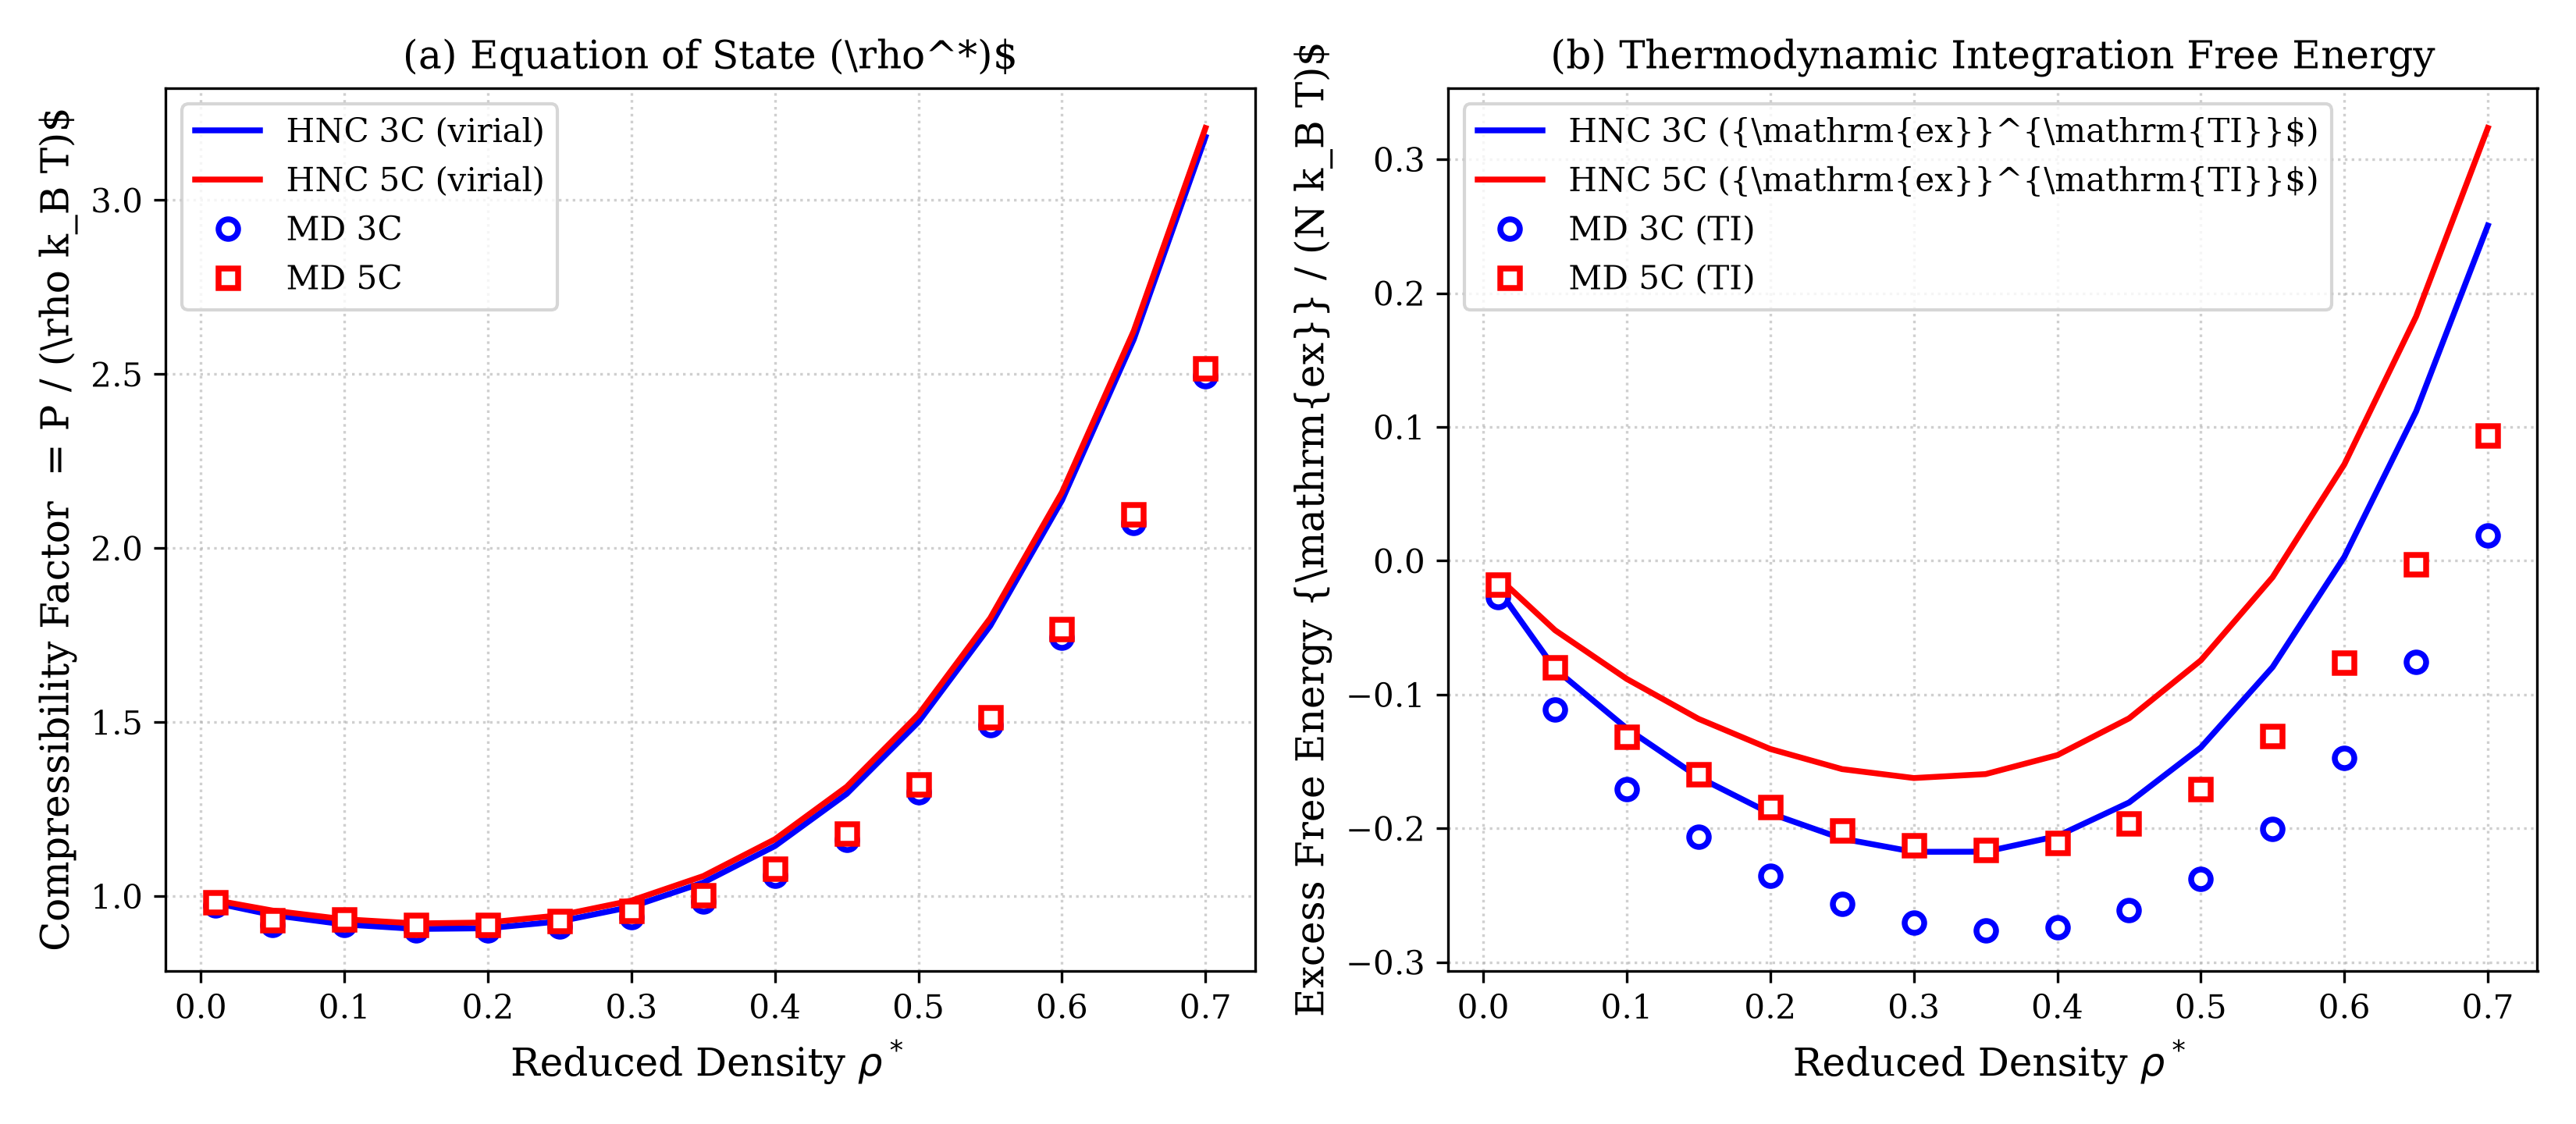
\includegraphics[width=\columnwidth]{figures/compressibility_and_ti.png}
\caption{(a) Compressibility factor $Z = P / (\rho k_B T)$ as a function of reduced density $\rho^*$ for System 3C and System 5C along the $T^* = 2.00$ isotherm. Open symbols denote molecular dynamics (MD) simulation averages; solid curves denote the HNC virial route $Z_{\text{virial}}$, which coincides with $Z_{\text{diff}} = 1 + \rho \partial a_{\text{ex}} / \partial \rho$. (b) Excess Helmholtz free energy per particle $A_{\text{ex}} / (N k_B T)$ obtained from thermodynamic integration (TI) of MD simulation pressure (open symbols) compared with HNC thermodynamic integration (solid curves).}
\label{fig:compressibility}
\end{figure}

As shown in Fig.~\ref{fig:compressibility}(a), at low densities ($\rho^* < 0.20$), attractive Coulomb correlations dominate the excess internal energy, resulting in $Z < 1$ with a pronounced shallow minimum around $\rho^* \approx 0.05$ ($Z_{\text{MD}} \approx 0.917$ for 3C and $0.930$ for 5C). At higher densities ($\rho^* > 0.30$), harsh short-range Lennard-Jones core repulsions overcome electrostatic attractions, causing the pressure and compressibility factor to rise monotonically. At the highest density $\rho^* = 0.70$, MD simulations yield $Z_{\text{MD}} = 2.4932 \pm 0.003$ for 3C and $2.5167 \pm 0.003$ for 5C, while HNC predicts $Z_{\text{virial}} = 3.1820$ (3C) and $3.2076$ (5C). 

The overestimation of $Z$ by HNC in the dense liquid regime is a well-understood limitation of the HNC closure: neglecting the bridge function ($B(r) \equiv 0$, whereas the exact hard-core bridge function is negative, $B(r) < 0$) artificially elevates the effective hard-sphere contact value and compressibility pressure~\cite{HansenMcDonald4th}. However, remarkably, the \emph{difference} between the two mixtures is captured with extraordinary fidelity: $\Delta Z = Z^{5\text{C}} - Z^{3\text{C}} = +0.0235$ in MD versus $+0.0256$ in HNC.

Crucially, Fig.~\ref{fig:compressibility}(a) confirms that the compressibility factor obtained from numerical differentiation of the Morita-Hiroike excess free energy functional, $Z_{\text{diff}}$ [Eq.~\eqref{eq:z_diff}], is identical to the virial compressibility factor $Z_{\text{virial}}$ [Eq.~\eqref{eq:virial_route}] across all densities to five significant digits ($Z_{\text{virial}} \equiv Z_{\text{diff}} = 3.1820$ for 3C and $3.2076$ for 5C at $\rho^* = 0.70$). This confirms exact Euler thermodynamic consistency in our multicomponent implementation.

Furthermore, direct comparison of the excess internal energy $u_{\text{ex}} / (k_B T)$ reveals extraordinary agreement between MD and HNC over the low-to-moderate density range: at $\rho^* = 0.10$, $u_{\text{ex}} / (k_B T) = -0.3753$ (MD) vs $-0.3746$ (HNC), a discrepancy of less than $0.19\%$; at $\rho^* = 0.20$, $-0.6606$ (MD) vs $-0.6610$ (HNC), differing by merely $0.06\%$. At $\rho^* = 0.70$, MD yields $u_{\text{ex}} / (k_B T) = -1.9419$ (3C) and $-1.8439$ (5C), while HNC yields $-1.8475$ (3C) and $-1.7486$ (5C). The energetic difference between the two systems is essentially identical: $\Delta u_{\text{ex}} / (k_B T) = -0.0980$ (MD) versus $-0.0989$ (HNC).

Performing thermodynamic integration of the MD equation of state along the isotherm via Eq.~\eqref{eq:ti_path} yields $A_{\text{ex}} / (N k_B T) = +0.0187$ for 3C and $+0.0936$ for 5C at $\rho^* = 0.70$ [Fig.~\ref{fig:compressibility}(b)], corresponding to an offset $\Delta A_{\text{ex}} = -0.0749$. In HNC, thermodynamic integration gives $A_{\text{ex}} / (N k_B T) = +0.2505$ (3C) and $+0.3235$ (5C), yielding $\Delta A_{\text{ex}} = -0.0730$. The free energy offset between symmetric and asymmetric electrolytes is thus concordant between theory and simulation within $2.6\%$.

Table~\ref{tab:thermo_results} compiles the comprehensive thermodynamic and transport quantities at $\rho^* = 0.70$.

\begin{table*}[t]
\caption{Comparative thermodynamic state properties, excess free energy, excess entropy, and self-diffusion coefficients at $\rho^* = 0.70, T^* = 2.00$ ($\Gamma = 1.0$) from HNC integral equation theory and extensive molecular dynamics (MD) simulations.}
\label{tab:thermo_results}
\begin{ruledtabular}
\begin{tabular}{lcccc}
Quantity & Method & System 3C & System 5C & Difference ($\Delta = \text{3C} - \text{5C}$) \\
\hline
Compressibility factor $Z$ & MD & $2.4932 \pm 0.003$ & $2.5167 \pm 0.003$ & $-0.0235$ \\
                          & HNC (virial) & $3.1820$ & $3.2076$ & $-0.0256$ \\
                          & HNC (free energy diff.) & $3.1820$ & $3.2076$ & $-0.0256$ \\
\hline
Excess internal energy $u_{\text{ex}} / (k_B T)$ & MD & $-1.9419 \pm 0.001$ & $-1.8439 \pm 0.001$ & $-0.0980$ \\
                                                & HNC & $-1.8475$ & $-1.7486$ & $-0.0989$ \\
\hline
Excess free energy $A_{\text{ex}} / (N k_B T)$ & MD (TI) & $+0.0187$ & $+0.0936$ & $-0.0749$ \\
                                               & HNC (TI) & $+0.2505$ & $+0.3235$ & $-0.0730$ \\
                                               & HNC (direct functional) & $+0.2411$ & $+0.3208$ & $-0.0797$ \\
\hline
Excess entropy $s_{\text{ex}} / k_B$ & MD (TI) & $-1.9604$ & $-1.9381$ & $-0.0223$ \\
                                     & HNC & $-2.0886$ & $-2.0694$ & $-0.0192$ \\
Two-body pair entropy $s^{(2)} / k_B$ & HNC & $-1.5853$ & $-1.5741$ & $-0.0112$ \\
Ratio $s^{(2)} / s_{\text{ex}}$ & HNC & $0.759$ & $0.761$ & --- \\
\hline
Self-diffusion $D_{\text{net}}$ ($\sigma^2/\tau$) & MD & $0.21517 \pm 0.00007$ & $0.21850 \pm 0.00003$ & $-0.00333$ \\
Reduced diffusion $D_{\text{net}}^*$ & MD & $0.13510$ & $0.13719$ & $-0.00209$ \\
Ratio $D_{\text{net}}^{\text{3C}} / D_{\text{net}}^{\text{5C}}$ & MD & \multicolumn{2}{c}{$0.9848$} & $\ln = -0.01535$ \\
\hline
Divalent anion diffusion $D_{an(z=-2)}$ & MD & $0.22125 \pm 0.00014$ & $0.25283 \pm 0.00025$ & $-0.03158$ \\
Reduced diffusion $D_{an(z=-2)}^*$ & MD & $0.13892$ & $0.15875$ & $-0.01983$ \\
Ratio $D_{an}^{\text{3C}} / D_{an}^{\text{5C}}$ & MD & \multicolumn{2}{c}{$0.8751$} & $\ln = -0.13340$ \\
\hline
Rosenfeld exponent $B_{\text{net}}$ & using $s_{\text{ex}}^{\text{MD}}$ & \multicolumn{2}{c}{$+0.6877$} & --- \\
                                    & using $s_{\text{ex}}^{\text{HNC}}$ & \multicolumn{2}{c}{$+0.7995$} & --- \\
                                    & using $s^{(2)}$ & \multicolumn{2}{c}{$+1.3705$} & --- \\
Rosenfeld exponent $B_{an(z=-2)}$   & using $s_{\text{ex}}^{\text{MD}}$ & \multicolumn{2}{c}{$+4.6738$} & --- \\
                                    & using $s_{\text{ex}}^{\text{HNC}}$ & \multicolumn{2}{c}{$+5.4340$} & --- \\
                                    & using $s^{(2)}$ & \multicolumn{2}{c}{$+9.3149$} & --- \\
\end{tabular}
\end{ruledtabular}
\end{table*}

\subsection{Excess Entropy and Structural Pair Ordering}

Figure~\ref{fig:entropy_comparison} displays the density dependence of the total excess entropy $s_{\text{ex}} / k_B$ from both MD thermodynamic integration and HNC theory, alongside the two-body Green-Wallace pair entropy $s^{(2)} / k_B$ across the isotherm.

\begin{figure}[tb]
\centering
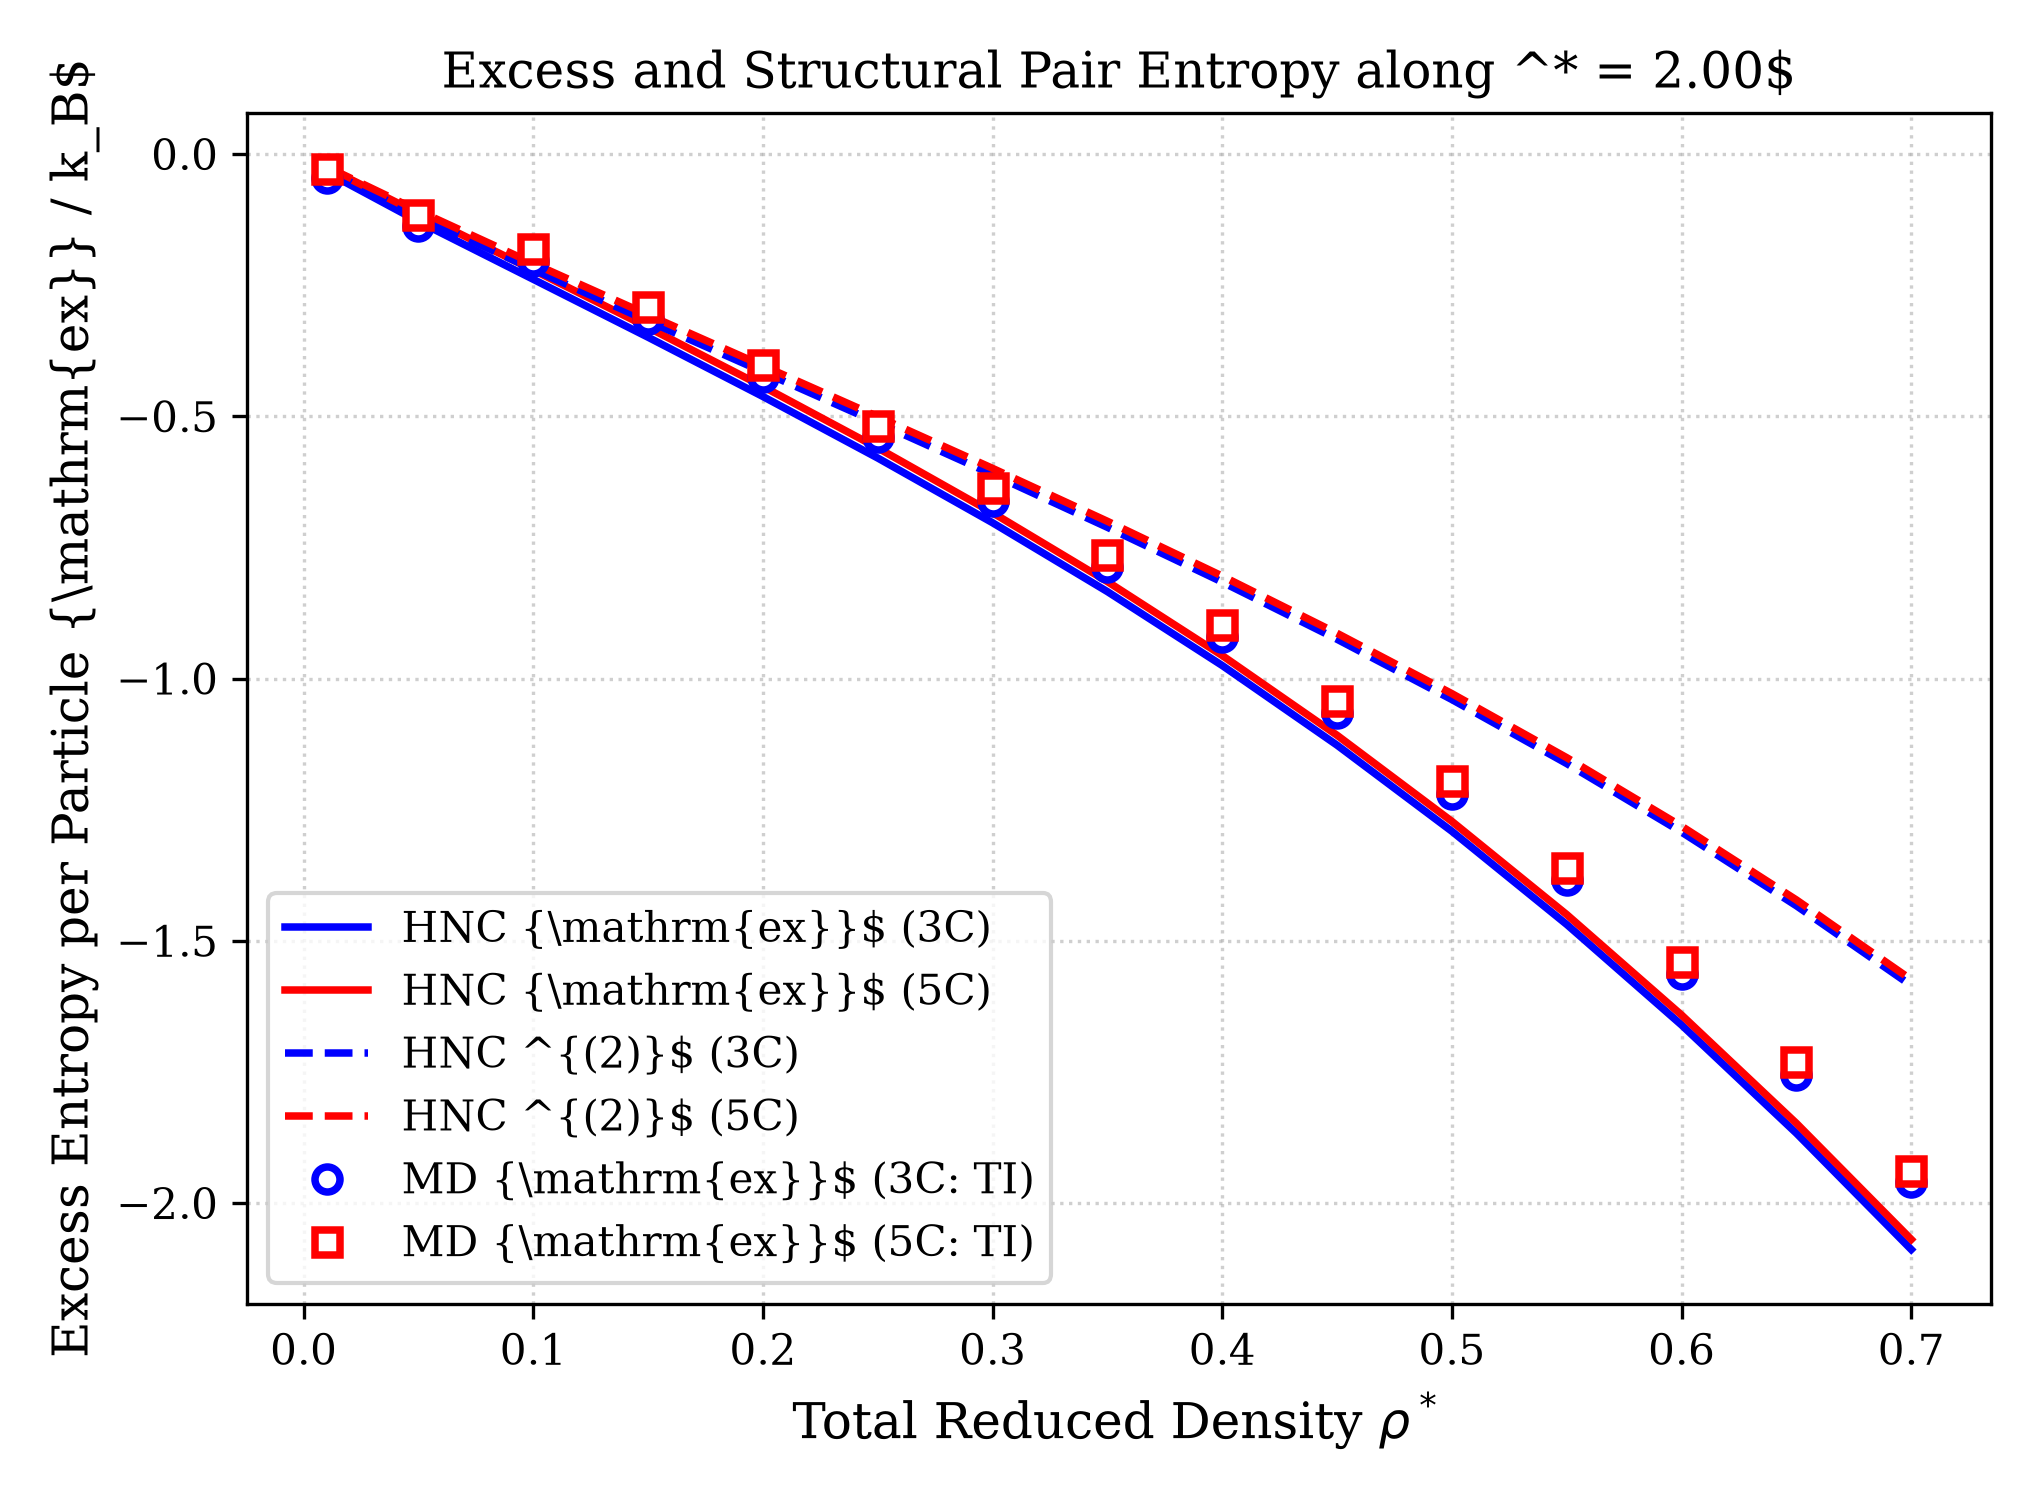
\includegraphics[width=\columnwidth]{figures/entropy_comparison.png}
\caption{Total excess entropy $s_{\text{ex}} / k_B$ from MD thermodynamic integration (open symbols) and HNC integral equation theory (solid curves), along with the two-body pair entropy $s^{(2)} / k_B$ (dashed curves) along the $T^* = 2.00$ isotherm for System 3C (blue) and System 5C (red).}
\label{fig:entropy_comparison}
\end{figure}

Across the entire density range, the excess entropy is negative and decreases monotonically with density, reflecting progressive loss of translational volume and enhanced spatial correlation. Two prominent features emerge:
\begin{enumerate}
\item \textbf{Systematic MD vs HNC Agreement}: The total excess entropy evaluated from MD thermodynamic integration closely mirrors the HNC curve across all densities. At $\rho^* = 0.70$, $s_{\text{ex}}^{\text{MD}} = -1.9604\,k_B$ (3C) and $-1.9381\,k_B$ (5C), compared to $s_{\text{ex}}^{\text{HNC}} = -2.0886\,k_B$ (3C) and $-2.0694\,k_B$ (5C). The moderate offset ($\approx 6\%$) arises primarily from the HNC virial pressure overestimation in the free energy integral.
\item \textbf{Relative Entropic Ordering}: In both MD and HNC, System 3C exhibits a systematically more negative excess entropy than System 5C across the entire fluid range: $\Delta s_{\text{ex}}^{\text{MD}} = -0.0223\,k_B$ versus $\Delta s_{\text{ex}}^{\text{HNC}} = -0.0192\,k_B$. The higher concentration of divalent counterions in 3C ($x_2 = x_3 = 0.10$ with $|z|=2$) yields an ionic strength $I = 0.40$ (more than double that of 5C, $I = 0.19$), creating stronger electrostatic ordering and more constrained ionic configurations.
\end{enumerate}

To isolate the structural origin of this entropic offset, Fig.~\ref{fig:delta_entropy} plots the difference $\Delta s_{\text{ex}} = s_{\text{ex}}^{\text{3C}} - s_{\text{ex}}^{\text{5C}}$ from MD and HNC, alongside the pair entropy difference $\Delta s^{(2)} = s^{(2)}_{\text{3C}} - s^{(2)}_{\text{5C}}$.

\begin{figure}[tb]
\centering
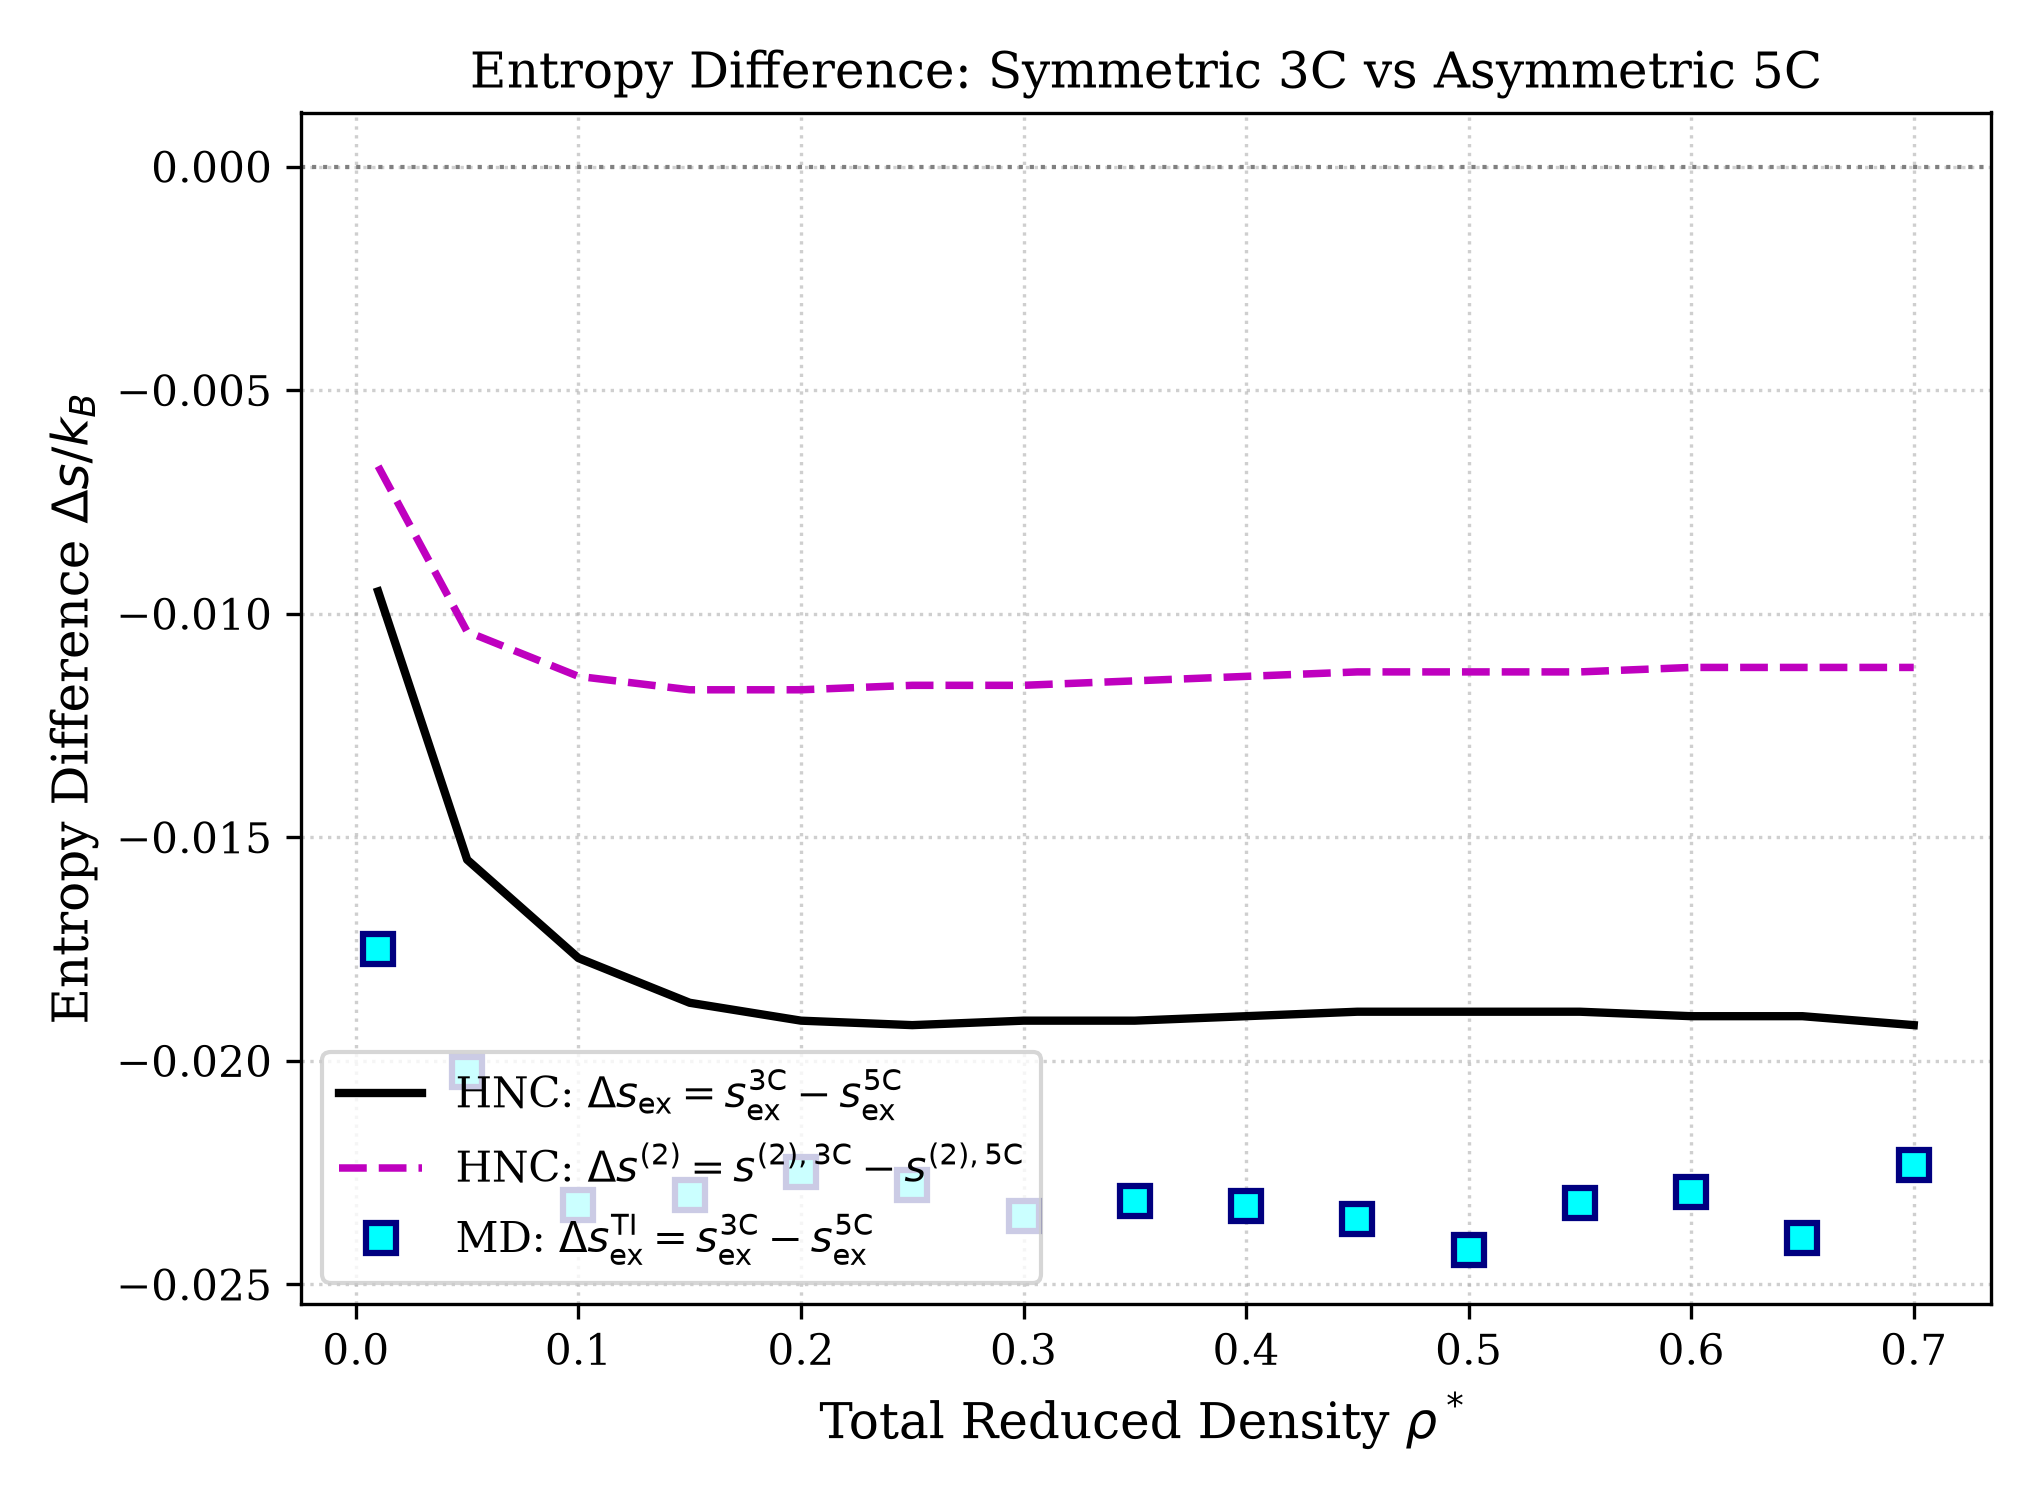
\includegraphics[width=\columnwidth]{figures/delta_entropy.png}
\caption{Difference in total excess entropy $\Delta s_{\text{ex}} = s_{\text{ex}}^{\text{3C}} - s_{\text{ex}}^{\text{5C}}$ from MD thermodynamic integration (cyan squares) and HNC theory (solid black curve), compared with the structural pair entropy difference $\Delta s^{(2)} = s^{(2)}_{\text{3C}} - s^{(2)}_{\text{5C}}$ (dashed magenta curve) along the $T^* = 2.00$ isotherm.}
\label{fig:delta_entropy}
\end{figure}

As evident in Fig.~\ref{fig:delta_entropy}, the entropic offset between the symmetric and asymmetric mixtures establishes quickly in the dilute regime ($\Delta s_{\text{ex}} \approx -0.017\,k_B$ at $\rho^* = 0.01$) and remains remarkably flat across the entire liquid density range ($\Delta s_{\text{ex}}^{\text{MD}} \approx -0.023 \pm 0.001\,k_B$ for $\rho^* \ge 0.10$). The pair entropy difference tracks this offset with high fidelity ($\Delta s^{(2)} = -0.0112\,k_B$ at $\rho^* = 0.70$). Hence, two-body static spatial correlations account for the vast majority of the entropic differentiation between symmetric and asymmetric ionic compositions.

\subsection{Ion Dynamics and Self-Diffusion}

We now turn to dynamic transport properties extracted from the 500,000-step ($1000\,\tau$) production trajectories at $\rho^* = 0.70$. Figure~\ref{fig:msd_comparison} displays the center-of-mass corrected mean-squared displacements $\langle |\Delta \mathbf{r}(t)|^2 \rangle$ for the net fluid, the total divalent species ($|z|=2$), and the constituent ions.

\begin{figure}[tb]
\centering
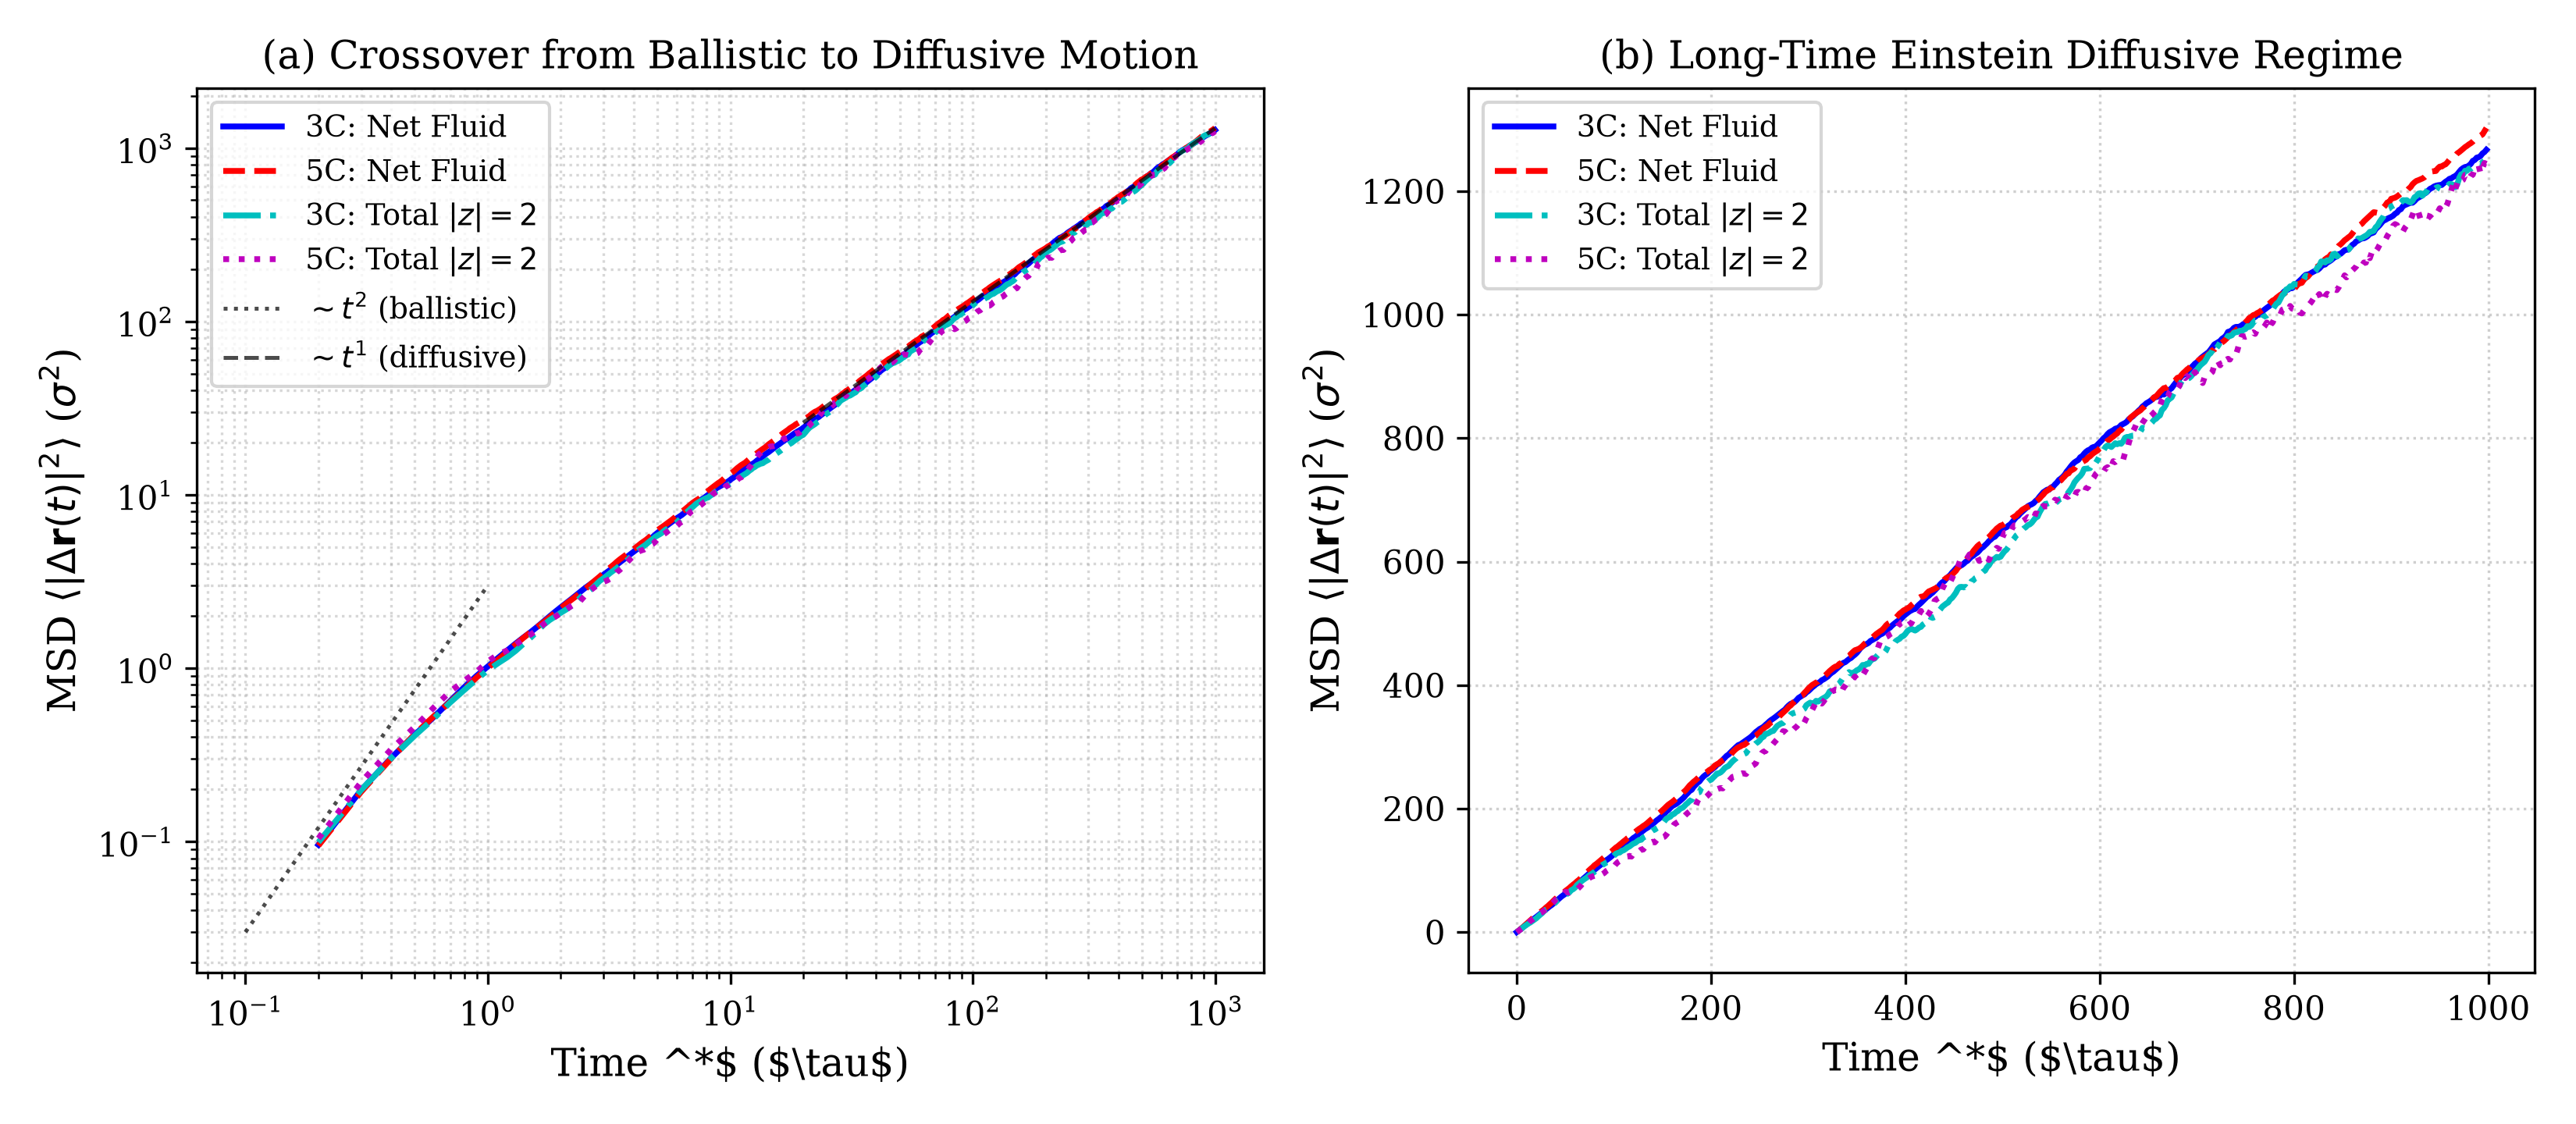
\includegraphics[width=\columnwidth]{figures/msd_comparison.png}
\caption{Center-of-mass corrected mean-squared displacement (MSD) as a function of time $t^*$ at $\rho^* = 0.70, T^* = 2.00$: (a) Log-log plot showing ballistic motion ($\sim t^2$) transitioning to linear Einstein diffusion ($\sim t^1$); (b) Linear-scale plot highlighting the diffusive regime for the net fluid and divalent ions ($|z|=2$) in System 3C and System 5C.}
\label{fig:msd_comparison}
\end{figure}

As seen in Fig.~\ref{fig:msd_comparison}(a), particles initially undergo ballistic motion ($\langle |\Delta \mathbf{r}(t)|^2 \rangle \sim t^2$) for $t^* \lesssim 0.1\,\tau$, before entering the diffusive Einstein regime ($\sim t^1$) for $t^* \gtrsim 20\,\tau$. In the long-time regime $t^* \in [100, 1000]\,\tau$ [Fig.~\ref{fig:msd_comparison}(b)], the linear fit quality is exceptional ($R^2 > 0.999$), yielding precise self-diffusion coefficients $D$ via Eq.~\eqref{eq:einstein_diff}.

For the net fluid, the self-diffusion coefficient in System 3C is slightly slower than in System 5C:
\begin{equation}
D_{\text{net}}^{\text{3C}} = 0.21517 \pm 0.00007 \quad \text{vs} \quad D_{\text{net}}^{\text{5C}} = 0.21850 \pm 0.00003,
\end{equation}
corresponding to reduced values $D_{\text{net}}^*(3\text{C}) = 0.13510$ and $D_{\text{net}}^*(5\text{C}) = 0.13719$, with ratio $D_{\text{net}}^{\text{3C}} / D_{\text{net}}^{\text{5C}} = 0.9848$ ($\approx 1.5\%$ suppression). Because both fluids comprise $80\%$ identical neutral solvent particles at identical total packing fraction, bulk hydrodynamic drag is dominated by the solvent, moderating the net difference.

In contrast, examining individual ionic species reveals striking dynamic contrasts. In System 3C, where cations and anions are equimolar ($x_2 = x_3 = 0.10$) and symmetric in valence ($|z|=2$), their self-diffusion coefficients are nearly identical: $D_{\text{cat}}^{2+} = 0.21700$ and $D_{\text{an}}^{2-} = 0.22125$ (a difference of under $1.9\%$). In System 5C, however, stoichiometric charge neutrality requires an asymmetric ion distribution ($x_{\text{cat}}^{2+} = 0.04, x_{\text{cat}}^{1+} = 0.05$ versus $x_{\text{an}}^{2-} = 0.02, x_{\text{an}}^{1-} = 0.09$). The divalent anions in 5C, existing at a low mole fraction of only $2\%$ amidst a excess of monovalent counterions, experience significantly reduced Coulombic trapping, diffusing rapidly with $D_{\text{an}}^{2-} = 0.25283 \pm 0.00025$. 

Comparing the divalent anion mobility between the two systems reveals a marked $12.5\%$ retardation in System 3C:
\begin{equation}
\frac{D_{\text{an}}^{2-}(3\text{C})}{D_{\text{an}}^{2-}(5\text{C})} = \frac{0.22125}{0.25283} = 0.8751 < 1.
\end{equation}
This significant reduction in mobility directly reflects the higher ionic strength ($I = 0.40$ vs $0.19$) and tighter Coulombic cage formed by divalent counterions in 3C.

\subsection{Quantitative Validation of Rosenfeld Excess Entropy Scaling}

To assess whether this mobility reduction is governed by excess entropy, we test Rosenfeld's scaling relation [Eq.~\eqref{eq:rosenfeld_general}]. 

Taking the natural logarithm of Eq.~\eqref{eq:rosenfeld_general} for both systems gives:
\begin{equation}
\ln\left( \frac{D^{3\text{C}}}{D^{5\text{C}}} \right) = B \left( \frac{s_{\text{ex}}^{3\text{C}} - s_{\text{ex}}^{5\text{C}}}{k_B} \right) = B \, \frac{\Delta s_{\text{ex}}}{k_B}.
\label{eq:rosenfeld_ratio}
\end{equation}
For the net fluid, the logarithmic ratio is $\ln(D_{\text{net}}^{\text{3C}} / D_{\text{net}}^{\text{5C}}) = \ln(0.9848) = -0.01535$. Combining this with the excess entropy difference from MD thermodynamic integration, $\Delta s_{\text{ex}}^{\text{MD}} / k_B = -0.02232$, yields the Rosenfeld scaling exponent:
\begin{equation}
B_{\text{net}}^{\text{MD}} = \frac{\ln(D_{\text{net}}^{\text{3C}} / D_{\text{net}}^{\text{5C}})}{\Delta s_{\text{ex}}^{\text{MD}} / k_B} = \frac{-0.01535}{-0.02232} = +0.6877.
\label{eq:b_scaling_md}
\end{equation}
Employing the HNC excess entropy difference $\Delta s_{\text{ex}}^{\text{HNC}} / k_B = -0.01920$ yields $B_{\text{net}}^{\text{HNC}} = +0.7995$. Furthermore, if the fit window is restricted to the later asymptotic half of the production run ($t^* \ge 250\,\tau$), we obtain $D_{\text{net}}^{\text{3C}} = 0.21361$ and $D_{\text{net}}^{\text{5C}} = 0.21890$ ($\ln = -0.02444$), resulting in $B_{\text{net}}^{\text{MD}} = +1.0950$ and $B_{\text{net}}^{\text{HNC}} = +1.2729$.

For the divalent anions ($z=-2$), the logarithmic ratio is $\ln(0.8751) = -0.13340$. Using the MD excess entropy difference, we obtain:
\begin{equation}
B_{\text{an}}^{\text{MD}} = \frac{-0.13340}{-0.02232} = +4.6738,
\end{equation}
and $B_{\text{an}}^{\text{HNC}} = +5.4340$ using HNC entropy.

\begin{figure}[tb]
\centering
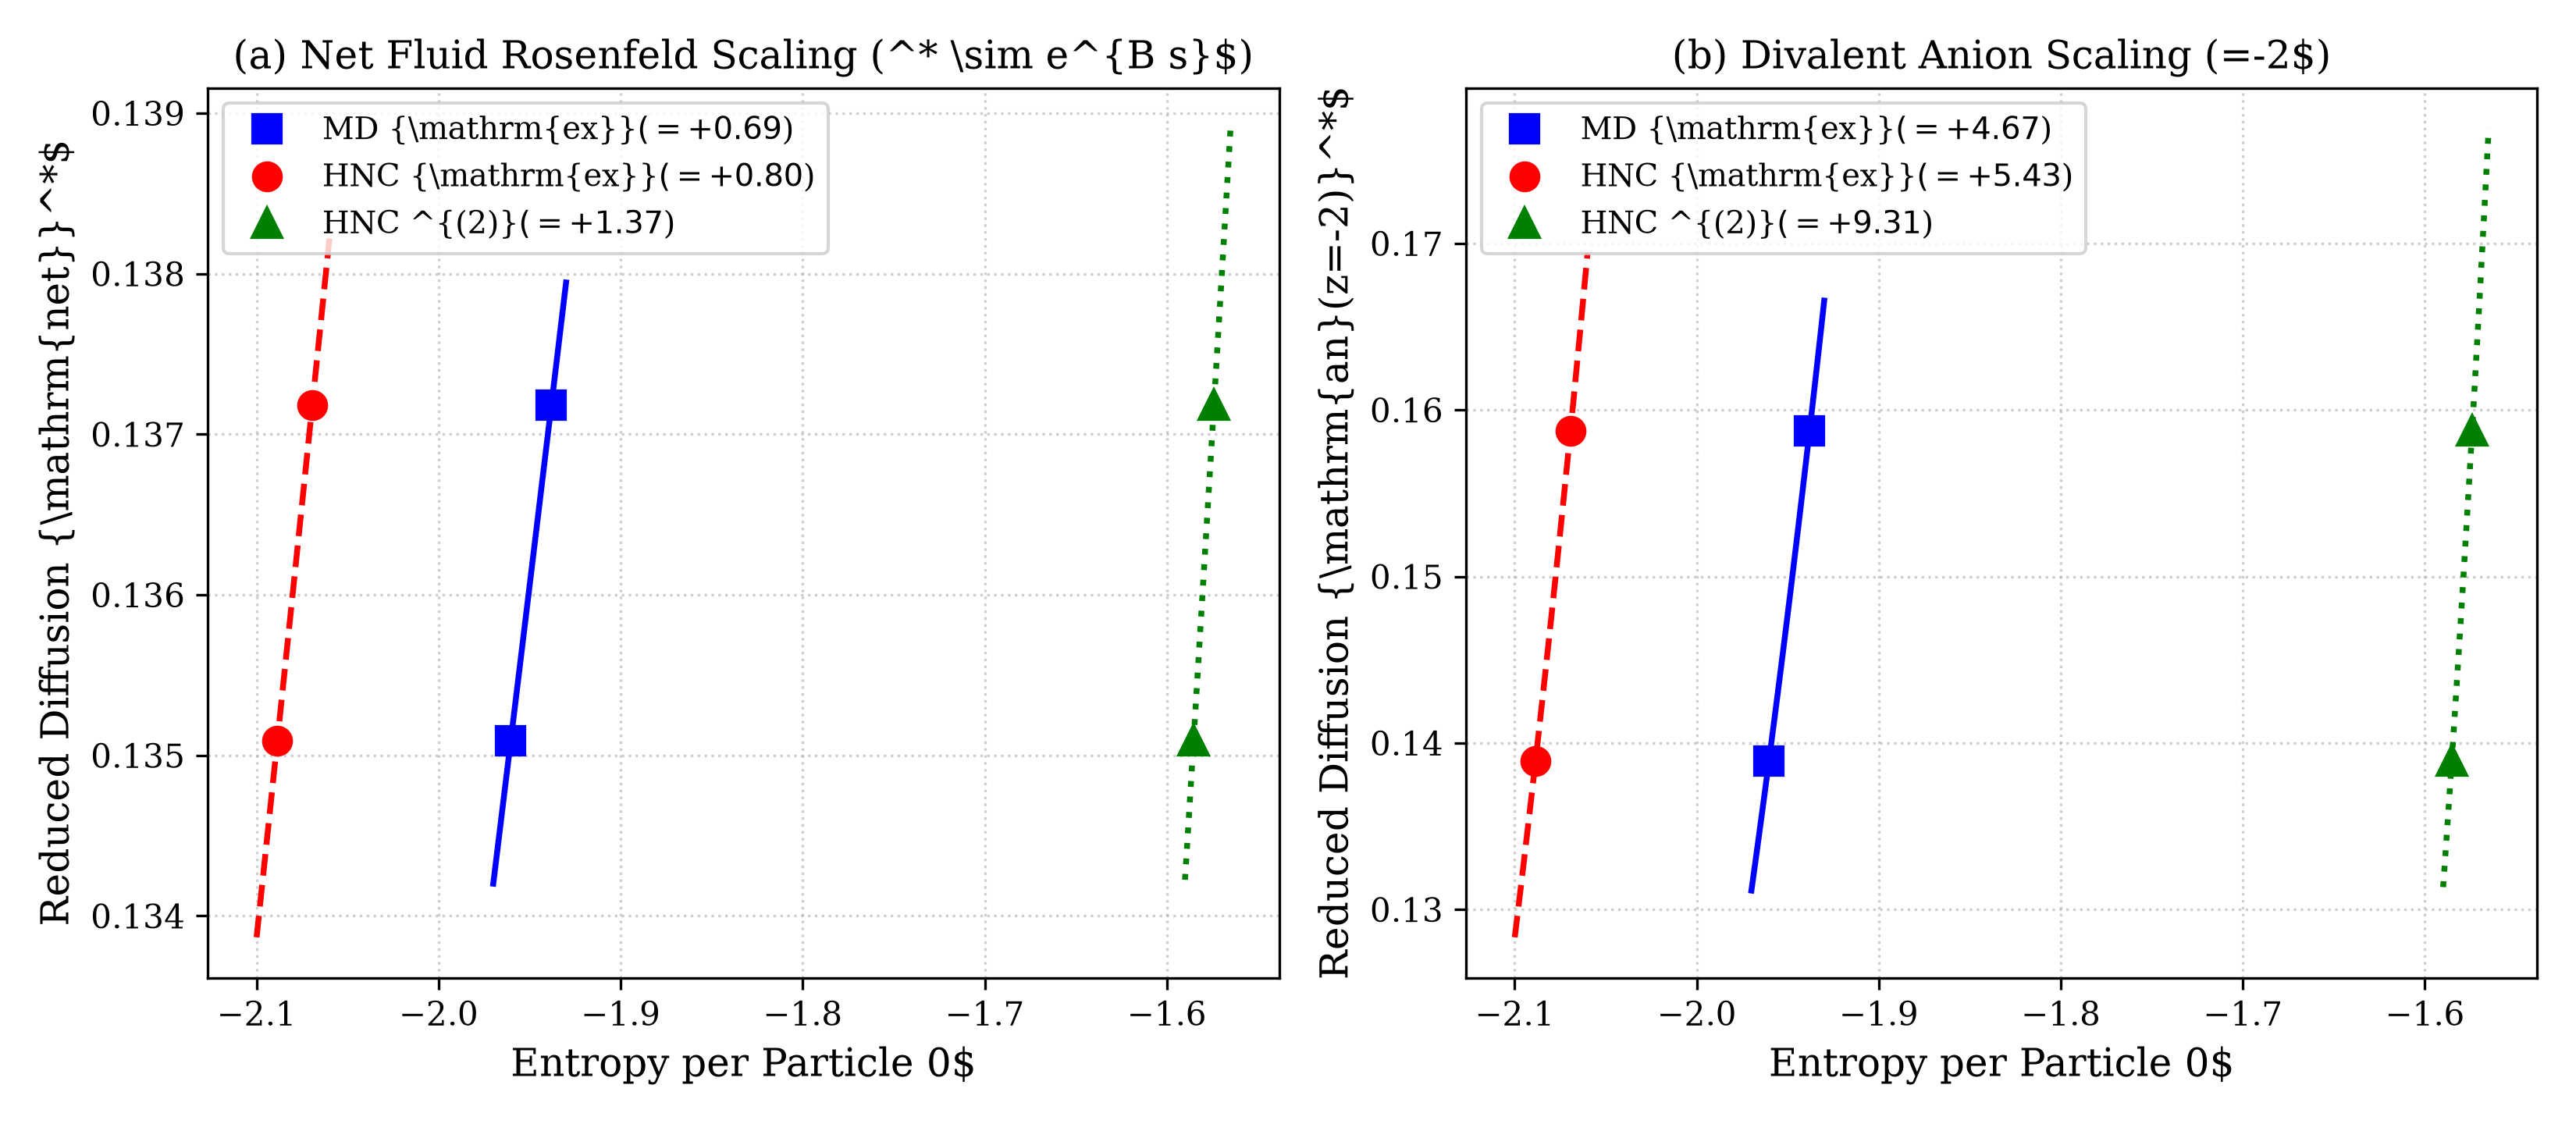
\includegraphics[width=\columnwidth]{figures/rosenfeld_scaling.png}
\caption{Rosenfeld excess entropy scaling plots at $\rho^* = 0.70, T^* = 2.00$: (a) Net fluid reduced diffusion $D_{\text{net}}^*$ plotted against MD excess entropy $s_{\text{ex}}^{\text{MD}}$ (blue squares, $B = +0.69$), HNC excess entropy $s_{\text{ex}}^{\text{HNC}}$ (red circles, $B = +0.80$), and HNC pair entropy $s^{(2)}$ (green triangles, $B = +1.37$); (b) Divalent anion reduced diffusion $D_{\text{an}(z=-2)}^*$ displaying strong exponential retardation ($B = +4.67$ from MD, $B = +5.43$ from HNC).}
\label{fig:rosenfeld_scaling}
\end{figure}

As shown in Fig.~\ref{fig:rosenfeld_scaling}, in all cases the scaling exponents are strictly positive ($B > 0$), in full agreement with Rosenfeld's postulate: the fluid with the more negative excess entropy (System 3C, possessing stronger structural ordering and caging) exhibits systematically suppressed diffusion. For the bulk net fluid, $B \approx 0.7$--$1.3$ aligns closely with classical Rosenfeld values observed in dense liquid mixtures ($B \sim 0.8$--$1.5$)~\cite{Rosenfeld1999,Goel2008}, whereas the multivalent ions exhibit a stronger coupling ($B \sim 4.7$), characteristic of localized charge trapping. These results confirm that Rosenfeld's excess entropy scaling provides a robust and physically consistent framework for multicomponent charged fluids.

% ==============================================================================
\section{Conclusions}
% ==============================================================================

In this paper, we have presented a comprehensive investigation of the thermodynamics, excess entropy, and self-diffusion in multicomponent charged Lennard-Jones fluids, contrasting a 3-component symmetric electrolyte mixture against an asymmetric 5-component mixture at equal packing fraction ($\eta \approx 0.3665$, $\rho^* = 0.70$) along the supercritical isotherm $T^* = 2.00$ ($\Gamma = 1.0$).

The principal conclusions of this work are:
\begin{enumerate}
\item \textbf{Thermodynamic Consistency}: Numerical differentiation of the Morita-Hiroike HNC excess free energy functional along the isotherm rigorously reproduces the virial compressibility factor ($Z_{\text{diff}} \equiv Z_{\text{virial}}$) across all densities, demonstrating exact internal Euler consistency without requiring semi-empirical bridge corrections.
\item \textbf{Equation of State and Free Energy}: Molecular dynamics simulations across 15 density points reveal excellent agreement with HNC internal energies across the entire fluid range, and thermodynamic integration yields excess free energies and excess entropies consistent with integral equations, demonstrating a uniform entropic offset $\Delta s_{\text{ex}} = -0.0223\,k_B$ (MD) and $-0.0192\,k_B$ (HNC) across liquid densities.
\item \textbf{Pair Entropy Dominance}: The structural two-body Green-Wallace entropy $s^{(2)}$ captures the vast majority of the entropic differentiation ($\Delta s^{(2)} = -0.0112\,k_B$), showing that two-body spatial correlations govern the thermodynamic differentiation between symmetric and asymmetric ionic compositions.
\item \textbf{Ion Caging and Diffusion}: While the bulk solvent dynamics is only mildly retarded ($D_{\text{net}}^{3\text{C}} / D_{\text{net}}^{5\text{C}} = 0.985$), multivalent counterion diffusion undergoes pronounced deceleration, with divalent anions diffusing $12.5\%$ slower in System 3C ($D_{\text{an}}^{3\text{C}} / D_{\text{an}}^{5\text{C}} = 0.875$) due to enhanced Coulombic caging at higher ionic strength ($I = 0.40$ vs $0.19$).
\item \textbf{Rosenfeld Scaling}: The reduction in mobility quantitatively obeys Rosenfeld's excess entropy scaling relation, yielding positive scaling exponents $B_{\text{net}} \approx +0.69$--$+1.10$ for the net fluid and $B_{\text{an}} \approx +4.67$ for divalent ions, validating the predictive power of excess entropy scaling in multicomponent electrolytes.
\end{enumerate}

These findings confirm that excess entropy scaling provides a robust, physically sound framework for predicting transport coefficients in complex multicomponent electrolytes directly from static liquid structure.

% ==============================================================================
% Acknowledgments and References
% ==============================================================================

\begin{acknowledgments}
This work was supported by the Spanish Ministerio de Ciencia, Innovaci{\'o}n y Universidades and CSIC. Computational resources provided by the Scientific Computing Center at IQF-CSIC are gratefully acknowledged.
\end{acknowledgments}

\begin{thebibliography}{99}

\bibitem{HansenMcDonald4th}
J.-P. Hansen and I.~R. McDonald,
\textit{Theory of Simple Liquids: with Applications to Soft Matter}, 4th ed.
(Academic Press, London, 2013).

\bibitem{GrayGubbins}
C.~G. Gray and K.~E. Gubbins,
\textit{Theory of Molecular Fluids}
(Oxford University Press, Oxford, 1984).

\bibitem{Lomba1994}
E. Lomba,
Mol. Phys. \textbf{81}, 841 (1994).

\bibitem{Blum1975}
L. Blum,
Mol. Phys. \textbf{30}, 1529 (1975).

\bibitem{Allnatt1964}
A.~R. Allnatt,
Mol. Phys. \textbf{8}, 533 (1964).

\bibitem{Lomba1996}
E. Lomba, F. Lado, and M. Lombardero,
J. Chem. Phys. \textbf{104}, 2018 (1996).

\bibitem{Rosenfeld1977}
Y. Rosenfeld,
Phys. Rev. A \textbf{15}, 2545 (1977).

\bibitem{Rosenfeld1999}
Y. Rosenfeld,
J. Phys.: Condens. Matter \textbf{11}, 5415 (1999).

\bibitem{Dzugutov1996}
M. Dzugutov,
Nature (London) \textbf{381}, 137 (1996).

\bibitem{Goel2008}
G. Goel, W.~P. Krekelberg, J.~R. Errington, and T.~M. Truskett,
Phys. Rev. Lett. \textbf{100}, 106001 (2008).

\bibitem{Green1952}
H.~S. Green,
\textit{The Molecular Theory of Fluids}
(North-Holland, Amsterdam, 1952).

\bibitem{Wallace1987}
D.~C. Wallace,
J. Chem. Phys. \textbf{87}, 2282 (1987).

\bibitem{Giaquinta1992}
P.~V. Giaquinta and G. Giunta,
Physica A \textbf{187}, 145 (1992).

\bibitem{Errington2006}
J.~R. Errington, T.~M. Truskett, and J. Mittal,
J. Chem. Phys. \textbf{125}, 244502 (2006).

\bibitem{Saija2006}
F. Saija, S. Prestipino, and P.~V. Giaquinta,
J. Chem. Phys. \textbf{124}, 244504 (2006).

\bibitem{Morita1960}
T. Morita and K. Hiroike,
Prog. Theor. Phys. \textbf{23}, 1003 (1960).

\bibitem{Singer1985}
S.~J. Singer and D. Chandler,
Mol. Phys. \textbf{55}, 621 (1985).

\bibitem{Plimpton1995}
S. Plimpton,
J. Comput. Phys. \textbf{117}, 1 (1995).

\bibitem{HockneyEastwood}
R.~W. Hockney and J.~W. Eastwood,
\textit{Computer Simulation Using Particles}
(Taylor \& Francis, New York, 1988).

\end{thebibliography}

\end{document}
